%%%%%%%%%%%%%%%%%%%%%%%%%%%%%%%%%%%%%%%%%%%%%%%%%%%%%%%%%%%%
%%% ELIFE ARTICLE TEMPLATE
%%%%%%%%%%%%%%%%%%%%%%%%%%%%%%%%%%%%%%%%%%%%%%%%%%%%%%%%%%%%
%%% PREAMBLE 
\documentclass[9pt,lineno]{elife}
% Use the onehalfspacing option for 1.5 line spacing
% Use the doublespacing option for 2.0 line spacing
% Please note that these options may affect formatting.
% Additionally, the use of the \newcommand function should be limited.


\usepackage{lipsum} % Required to insert dummy text
\usepackage[version=4]{mhchem}
\usepackage{siunitx}
\DeclareSIUnit\Molar{M}

%%%%%%%%%%%%%%%%%%%%%%%%%%%%%%%%%%%%%%%%%%%%%%%%%%%%%%%%%%%%
%%% CUSTOM PACKAGES
%%%%%%%%%%%%%%%%%%%%%%%%%%%%%%%%%%%%%%%%%%%%%%%%%%%%%%%%%%%%

% Required to draw Fig. 1
\usepackage{tikz}
\usetikzlibrary{decorations.pathmorphing}
\usetikzlibrary{shapes.symbols}
\usepackage{helvet}

% Proof commands
\usepackage{amsthm}
\newtheorem{lemma}{Lemma}
\newcommand{\Z}{\mathbb{Z}}
\newcommand{\C}{\mathbb{C}}
\newcommand{\R}{\mathbb{R}}
\newcommand{\N}{\mathbb{N}}
\newcommand{\Q}{\mathbb{Q}}

% Vim macro to remove color or sout commands:
% 1. place cursor at \ before command
% 2. type "q-d-d-t-{-%-x-ctrl-o-x-q"
% Test:
%\label{pi-silencing}


%%%%%%%%%%%%%%%%%%%%%%%%%%%%%%%%%%%%%%%%%%%%%%%%%%%%%%%%%%%%
%%% ARTICLE SETUP
%%%%%%%%%%%%%%%%%%%%%%%%%%%%%%%%%%%%%%%%%%%%%%%%%%%%%%%%%%%%

\title{Muller's Ratchet in Asexual Populations Doomed to Extinction}

\author[1]{Logan Chipkin}
\author[2,3]{Peter Olofsson}
\author[2]{Ryan C.\ Daileda}
\author[1*]{Ricardo B.\ R.\ Azevedo}
\affil[1]{Department of Biology \& Biochemistry, University of Houston, Houston, Texas, U.S.A.}
\affil[2]{Department of Mathematics, Trinity University, San Antonio, Texas, U.S.A.}
\affil[3]{Department of Mathematics, Physics and Chemical Engineering, Jönköping University, Sweden}

\corr{razevedo@uh.edu}{}


%%%%%%%%%%%%%%%%%%%%%%%%%%%%%%%%%%%%%%%%%%%%%%%%%%%%%%%%%%%%
%%% ARTICLE START
%%%%%%%%%%%%%%%%%%%%%%%%%%%%%%%%%%%%%%%%%%%%%%%%%%%%%%%%%%%%

\begin{document}




\maketitle




\begin{abstract}
%Please provide an abstract of no more than 150 words. Your abstract should explain the main contributions of your article, and should not contain any material that is not included in the main text.
Asexual populations are expected to accumulate deleterious mutations through a process known as Muller's Ratchet.  Lynch, Gabriel, and colleagues have proposed that the Ratchet eventually results in a vicious cycle of mutation accumulation and population decline that drives populations to extinction.  They called this phenomenon mutational meltdown.  Here, we analyze the  meltdown using a multitype branching process model where, in the presence of mutation, populations are doomed to extinction.  We find that extinction occurs more quickly in small populations, experiencing a high deleterious mutation rate, and mutations with more severe deleterious effects.  The effects of mutational parameters on extinction time in doomed populations differ from those on the severity of Muller's Ratchet in populations of constant size.  We also find that mutational meltdown, although it does occur in our model, does not determine extinction time.  Rather, extinction time is determined by the expected impact of deleterious mutations on fitness.
\end{abstract}




\section{Introduction}




\medskip

\begin{quotation}
``All populations are doomed to eventual extinction.'' \citet{Lynch_MUTATION_1990}
\end{quotation}

\noindent
In the absence of back mutations, an asexual individual cannot produce offspring carrying fewer deleterious mutations than itself. Indeed, it is always possible that individual offspring will accrue additional deleterious mutations. 
As a result, the class of individuals with the fewest deleterious mutations may, by chance, disappear irreversibly from the population, a process known as Muller's Ratchet
\citep{Muller_The_1964, Felsenstein_The_1974, Haigh_The_1978}.  Successive ``clicks'' of the Ratchet will cause the fitness of asexual populations to decline.
Muller's Ratchet has been invoked to explain 
the evolution of sex \citep{Muller_The_1964, Felsenstein_The_1974, gor08},
the extinction of small populations \citep{lyn93, lyn95},
the accelerated rate of evolution of endosymbiotic bacteria \citep{mor96},
the degeneration of Y-chromosomes \citep{Charlesworth_Model_1978, gor00b},
and cancer progression \citep{McFarland_Impact_2013, McFarland_Tug_2014}.  

\citet{Haigh_The_1978} argued that the Ratchet should click at a rate inversely proportional to the size of the least-loaded class in a population.  If $k$ is the lowest number of deleterious mutations present in an individual in the population, 
the size of the least-loaded class at mutation-selection-drift equilibrium is
%
\begin{equation}
  \hat n_k = N e^{-U/s} \quad ,
  \label{eq:haigh}
\end{equation}
%
where $N$ is the size of the population, $U$ is the 
expected number of deleterious mutations
per genome per generation, and $s$ is the deleterious effect of a mutation. 
Haigh suggested that genetic drift causes the actual value of $n_k$ to deviate stochastically from $\hat n_k$.  The smaller the value of $\hat n_k$, the greater the probability that $n_k$ will hit zero, causing the Ratchet to click.  
If $\hat n_k > 1$, then after a click of the Ratchet, the size of the new least-loaded class will go to a new equilibrium, $\hat n_{k+1}$, equal to $\hat n_k$ in \EQ{haigh}. 
Haigh concluded that Muller's Ratchet should click faster 
in small populations, 
experiencing a high deleterious mutation rate, 
and mutations with milder deleterious effects (low $s$).
Subsequent work has derived more accurate estimates of the rate of clicking of the Ratchet, both when $\hat n_k > 1$ \citep{Stephan_The_1993, Gordo_On_2000, gor00b, Neher_Fluctuations_2012, met13} and when $\hat n_k < 1$ \citep{Gessler_The_1995, Rouzine_The_2003, Rouzine_The_2008}. 

Beginning with Haigh's foundational study, most research on Muller's Ratchet has assumed that 
the size of a population remains constant as deleterious mutations accumulate \citep[e.g.,][]{Gessler_The_1995, Gordo_On_2000, gor00b, Rouzine_The_2003, met13}.  
This assumption is biologically unrealistic---if true, fitness would decline continuously but the population would be immortal \citep{Lynch_MUTATION_1990, mel91}.  Lynch, Gabriel, and colleagues studied more realistic models where the fitness of an individual influences its fertility and populations experience density-dependent regulation \citep{Lynch_MUTATION_1990, lyn93, Gabriel_MULLER_1993, lyn95}.  They found that Muller's Ratchet causes population size to decline, which accelerates the Ratchet, which further reduces population size.  This positive feedback results in a ``mutational meltdown'' that drives the population to extinction \citep{Lynch_MUTATION_1990, lyn93, Gabriel_MULLER_1993}. 

In one model, \citet{lyn93} considered a population of asexual organisms subject to a carrying capacity of $\widehat N$ individuals.  Each individual produces $R$ offspring.  The number of mutations is Poisson distributed with rate $U$.  The offspring then undergo viability selection with a probability of survival
%
\begin{equation}
  w_k=(1-s)^{k} \quad ,
  \label{eq:fit}
\end{equation}
%
where
$k \geq 0$ is the number of deleterious mutations in the individual offspring,  
and $0 < s < 1$ is the deleterious effect of each mutation. 
If the number of offspring surviving viability selection is $N' > \widehat N$, $N' - \widehat N$ individuals die and $\widehat N$ individuals survive, independently of their fitness; if $N' \leq \widehat N$, all $N'$ individuals survive.  
Reproduction occurs after viability selection and density-dependent regulation.  Assuming that initially all individuals in the population are mutation-free and that $N R > \widehat N$, Muller's Ratchet proceeds in three phases in this model.  
%
First, mutations enter the population and accumulate rapidly.  As the distribution of mutation numbers approaches mutation-selection-drift equilibrium mutation accumulation slows down.
%
Second, the rate of mutation accumulation settles into a steady rate.  This phase proceeds as in the classic constant population size model of Muller's Ratchet \citep{Haigh_The_1978} and lasts while $N R \, \overline w \gtrsim \widehat N$.
%
Third, when mean viability reaches $\overline w = 1/R$ (i.e., when $N R \, \overline w = \widehat N$) the population size begins to decline, triggering mutational meltdown.  During this phase the population is doomed to extinction.


\citet{lyn93} derived some analytical expressions to describe the dynamics of mutation accumulation during the first two phases and the times at which these two phases end.  
However, they did not present any analytical theory on the dynamics or duration of the third (meltdown) phase itself \citep[see also][]{Gabriel_MULLER_1993, lyn95}.
Thus, the validity of the Lynch-Gabriel view of the mutational meltdown is difficult to evaluate.
%
Here we model the mutational meltdown phase of Muller's Ratchet using a multitype branching process.
We derive an analytical approximation for the expected time to extinction under this model
of populations doomed to extinction.  
We find that extinction occurs more quickly in small populations, 
experiencing a high deleterious mutation rate $(u)$, 
and mutations with \emph{more severe} deleterious effects (high $s$).  
Our results differ from predictions on the relationship between the severity of Muller's Ratchet and mutational parameters in populations of constant size.
We also find that mutational meltdown, 
although it does occur in doomed populations,
is not an important determinant of time to extinction. 
Rather, extinction time is approximately inversely proportional to the product $us$, that is, 
the expected impact of deleterious mutations on fitness.


\begin{figure}[!ht]
  \centering
	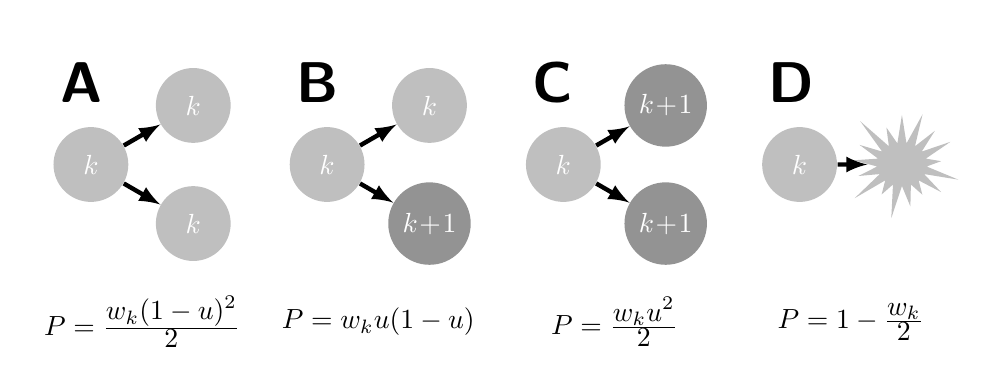
\begin{tikzpicture} 
% Row 1
		\node (par1)       at       (0, 0)       [circle, minimum size=9.5mm, fill=gray!50]      {\textcolor{white}{$k$}};
		\node (off11)      at       (1.3, .75)   [circle, minimum size=9.5mm, fill=gray!50]      {\textcolor{white}{$k$}};
		\node (off12)      at       (1.3, -.75)  [circle, minimum size=9.5mm, fill=gray!50]      {\textcolor{white}{$k$}};
		\draw[-latex, ultra thick]  (par1)  to  (off11);
		\draw[-latex, ultra thick]  (par1)  to  (off12);
		\node (par2)       at       (3, 0)       [circle, minimum size=9.5mm, fill=gray!50]      {\textcolor{white}{$k$}};
		\node (off21)      at       (4.3, .75)   [circle, minimum size=9.5mm, fill=gray!50]      {\textcolor{white}{$k$}};
		\node (off22)      at       (4.3, -.75)  [circle, minimum size=9.5mm,fill=gray!85]      {\textcolor{white}{$k\!+\!1$}};
		\draw[-latex, ultra thick]  (par2)  to  (off21);
		\draw[-latex, ultra thick]  (par2)  to  (off22);
        \node (par3)       at       (6, 0)       [circle, minimum size=9.5mm, fill=gray!50]      {\textcolor{white}{$k$}};
		\node (off31)      at       (7.3, .75)   [circle, minimum size=9.5mm, fill=gray!85]      {\textcolor{white}{$k\!+\!1$}};
		\node (off32)      at       (7.3, -.75)  [circle, minimum size=9.5mm, fill=gray!85]      {\textcolor{white}{$k\!+\!1$}};
		\draw[-latex, ultra thick]  (par3)  to  (off31);
		\draw[-latex, ultra thick]  (par3)  to  (off32);
        \node (ind)        at       (9, 0)       [circle, minimum size=9.5mm, fill=gray!50]      {\textcolor{white}{$k$}};
        \node (dead)       at       (10.3, 0)    [starburst, minimum size=3mm, fill=gray!50]      {\textcolor{gray!50}{$n$}};
        \draw[-latex, ultra thick]  (ind)  to  (dead);
% Row 2
		\node (p1)  at       (0.65, -2)      {$P = \frac{\displaystyle w_k (1-u)^2}{\displaystyle 2}$};
		\node (p2)  at       (3.65, -2)      {$P = w_k u (1-u)$};
        \node (p3)  at       (6.65, -2)      {$P = \frac{\displaystyle w_k u^2}{\displaystyle 2}$};
        \node (p4)  at       (9.65, -2)      {$P = 1-\frac{\displaystyle w_k}{\displaystyle 2}$};
% Labels
\huge
		\node[right] (A)          at       (-.81, 1.04) [circle]  {\sf\textbf{A}};
		\node[right] (B)          at       (2.19, 1.04) [circle]  {\sf\textbf{B}};
		\node[right] (C)          at       (5.19, 1.04) [circle]  {\sf\textbf{C}};
		\node[right] (D)          at       (8.19, 1.04) [circle]  {\sf\textbf{D}};
	\end{tikzpicture}	

 	\caption{Multitype branching process.  At each time step, an individual of type $k$---i.e, with $k$ deleterious mutations (light gray)---can have one of four fates \textbf{(A--D)} with different probabilities, $P$ (see \TABLE{pars}).  
%
It can either die \textbf{(D)} or survive and split into two daughters \textbf{(A--C)}. 
%
The daughters inherit the $k$ mutations from their mother.
A daughter can acquire one additional mutation and become a type $k+1$ individual (dark gray) \textbf{(B--C)}.}
	\label{fig:branching}	
\end{figure}




\section{Model}




\subsection{Branching process}

A population consists of $N_k$ individuals with $k=0,\, 1,\, 2,\, \ldots$ deleterious mutations.  Below, we refer to individuals with $k$ deleterious mutations as belonging to type $k$.

The size $N = \sum_i N_i$ of the population is allowed to change according to a discrete-time branching process.   
Each generation, an individual of type $k$ reproduces by splitting into two daughters with probability $w_k/2$ and dies with probability $1 - w_k/2$ (\FIG{branching}), where $w_k$ is the 
expected number of offspring 
of an individual of type $k$---i.e., its  \textit{absolute} fitness (\EQ{fit}). 
We assume that all mutations have the same deleterious effect $s$ and do not interact epistatically.  

Any offspring may acquire one deleterious mutation with probability $u$. 
Note that $u$ is defined differently from the mutation rate, $U$, in Haigh's model (\EQ{haigh}).
The number of mutant offspring of a surviving individual of any type is binomially distributed  with parameters $2$ and $u$ (\FIG{branching}).

This branching process
yields the probability generating function (p.g.f.) of the number of $k$-type offspring of a $k$-type individual 
%
\begin{equation}
  \varphi_{k}(x)=1-\frac{w_k}{2}\left(1-u^2-2u(1\!-\!u)x-(1\!-\!u)^2x^2\right)
  \label{eq:pgf}
\end{equation}
%
and mean reproduction matrix $M$ with entries 
%
\begin{equation}
  \left\{\begin{array}{lll}
            m_{k,k} & = & w_k (1-u)\\
            m_{k,k+1} & = & w_k u\\
            \end{array} \right.
  \label{eq:m}
\end{equation}
%
where $m_{i,j}$ is the expected number of offspring of type $j$ generated by an individual of type $i$.  All other entries of $M$ are 0.

The mean reproduction matrix for generation $t$ is $M^{t}$, the $t$-th power of $M$. For any $t$, all entries of $M^{t}$ below the diagonal are 0. 
Assuming the fitness function in \EQ{fit}, we can get an explicit form for the entries $m_{i,j}^{(t)}$ of $M^{t}$:
%
\begin{equation}
  m^{(t)}_{k,k+j} = \displaystyle (1-u)^{t-j} u^{j}(1 - s)^{tk\,+\textstyle\frac{j(j-1)}{2}}\prod_{i=1}^{j}\frac{1 - (1 - s)^{t+1-i}}{1 - (1 - s)^{i}}
  \label{eq:mt}
\end{equation}
where $j=0,\,1,\,2,\,\ldots\;$
% 
For a proof, see \autoref{app:proof}.  




\begin{table}[!ht]
\caption{\label{tab:pars}Variables and parameters.}
\begin{tabular}{S l}
\toprule
Symbol         & Description     \\
\midrule
$u$            & Probability that an individual acquires a deleterious mutation (\FIG{branching}).\\
$s$            & Deleterious effect of a mutation (\EQ{fit}).\\
$w_k$          & Fitness of an individual of type $k$, i.e.\ with $k$ deleterious mutations (\EQ{fit}).\\
$m_{i, j}$     & Expected number of offspring of type $j$ generated by an individual of type $i$ \\
               & (\EQ{m}).\\
$n_{0}$        & Initial number of mutation-free individuals in the population.\\
$n_k$          & Expected number of $k$-type individuals in the population.\\
$N$            & Total population size (\EQ{N}).\\
$t_k$          & Expected extinction time of $k$-type individuals in generations, i.e.\ the $k$-th click of the \\
               & Ratchet (\EQ{tk}).\\
$\Delta t_k$   & Interval between clicks $k-1$ and $k$ of the Ratchet (\EQ{deltat}).\\
$x_k$          & Expected number of $k$-type individuals at the extinction time of type $k-1$ \\
               & (\EQ{xk}).\\
$\mathbf{T}$   & Expected extinction time of the entire population in generations (\EQ{T}).\\
\bottomrule
\end{tabular}
\end{table}


\subsection{Extinction time of individuals of type \emph{k}}


Let $\tau_k$ denote the time of extinction of individuals of type $k$ in a population started from $N_{k}$ ancestors of type $k$ where $N_k$ is a random variable on $\{0,1,2,...\}$ (if $N_k=0$, then $\tau_k=0$).  
There are no individuals of type $i < k$ in the population.
By a standard result from probability theory
%
\[ E[\tau_k]=\sum_{t=0}^{\infty}P(\tau_k>t) \quad . \]

The time of extinction of the entire type-$k$ subpopulation is the time of extinction of the $N_{k}$ independent subpopulations started from the ancestors. The p.g.f.\ of the number of $k$-type individuals in generation $t$ is given by the $t$-fold composition of $\varphi_k$ (\EQ{pgf}) with itself, denoted by $\varphi^{(t)}_k$. We get
%
\[ \tau_{k}=\max\{\tau_{k,1},...,\tau_{k,N_{k}}\} \]   
%
where $\tau_{k,j}$ is the time of extinction of the subpopulation started from the $j$th individual, $j=1,...,N_k$. If we let $Z_{t}^{(k,j)}$ denote the number of type-$k$ individuals in generation $t$ stemming from the $j$th individual we have the equivalence 
%
\[ \tau_{k,j}\leq t \; \Leftrightarrow \; Z_{t}^{(k,j)}=0 \]
%
and get the conditional probability given $N_k$

\begin{align*}
%
P(\tau_{k}>t|N_k) & =  1-P(\tau_{k}\leq t|N_k)\\[3pt]
           & =  1-\prod_{j=1}^{N_{k}}P(\tau_{k,j}\leq t)\\[3pt]
           & =  1-\left(\varphi_{k}^{(t)}(0)\right)^{N_{k}}
\end{align*}
%
for $t>0$ which gives 
%
\[ E[\tau_{k}] = P(\tau_{k}>0) + E\left[\sum_{t=1}^{\infty}\left(1-\left(\varphi_{k}^{(t)}(0)\right)^{N_{k}}\right)\right] \]

With $n_k=E[N_k]$, a first-order Taylor approximation gives 
%
\begin{equation}
%
E[\tau_{k}] \approx P(\tau_{k}>0) + \sum_{t=1}^{\infty}\left(1-\left(\varphi_{k}^{(t)}(0)\right)^{n_{k}}\right)
%
\label{eq:tauk}
\end{equation}
%
Note that for $k=0$ we have $P(\tau_{0}>0)=1$ because there are always individuals present at time $0$. For $k>0$, however, we have $P(\tau_{k}>0)<1$ because, for example, 
the entire population may already be extinct in generation 1. 

In a similar way, we get the variance as
%
\begin{equation}
\mathrm{Var}[\tau_{k}]=E[\tau_{k}(\tau_{k}-1)]+E[\tau_{k}]-E^{2}[\tau_{k}]
\label{eq:vartauk}
\end{equation}
%
where

\begin{align*}
%
E[\tau_{k}(\tau_{k}-1)] & =  2\sum_{t=1}^{\infty}tP(\tau_{k}>t)\\[5pt]
& \approx  2\sum_{t=1}^{\infty}t\left(1-\left(\varphi_{k}^{(t)}(0)\right)^{n_k}\right)
%
\end{align*}


\subsection{Extinction time of the entire population}


By well-known results from the theory of branching processes, the extinction time of the entire population has finite mean only in the {\em subcritical} case, that is, when the mean number of offspring per individual is less than 1. 
The expected number of offspring of type $k$ produced by an individual of type $k$ is $m_{k,k}$ (\EQ{m}).  
If $m_{k,k}=1$ (the \emph{critical} case), the extinction time $\tau_k$ is finite but has an infinite mean and if $m_{k,k} > 1$ (the {\em supercritical} case), $\tau_k$ itself may assume the value $\infty$.  

\EQ{m} shows that $m_{k,k} < 1$ (the {\em subcritical} case) for individuals of any type $k$ provided all mutations are deleterious $(0<s<1)$ and the mutation rate is nonzero $(u>0)$.  Thus, the expected extinction time of every type $k$ is finite.  
In other words, the population is doomed to eventual extinction.

Start with a fixed number $n_{0}$ of mutation-free individuals and denote by $T_{0}$ the time (generation) of extinction of this class. Conditioned on $T_{0}$, the expected number of individuals in class 1 (those with $k=1$ mutation) is therefore $m_{0,1}^{(T_0)}$
(see \EQ{mt})
which we note is a function of the random variable $T_{0}$. Thus, the expected number of individuals in class 1 at the time of extinction of class 0 is obtained by taking the expected value in $m_{0,1}^{(T_0)}$. To this end, recall \EQ{mt} and define the function 
%
\[ g_1(\cdot)=m_{0,1}^{(\cdot)} \]
%
so that 

\begin{align*}
%
E\left[m_{0,1}^{(T_{0})}\right] &=  E[g_{1}(T_{0})]\\
&\approx  g_{1}\left(E[T_{0}]\right)
%
\end{align*}
%
where we use a first-order Taylor approximation. To generalize the idea, we define the expected number of descendants of type $j$ from a mutation-free individual after $t$ generations
%
\begin{equation}
g_{j}(t) = \left\{\begin{array}{lll}
%
    0              & , & t<j       \\ [4pt]
	m^{(t)}_{0, j} & , & t \geq j
    \end{array}
%
\right. 
\label{eq:gj}
\end{equation}
%
(see \EQ{mt}).


Now let $T_{k}$ be the extinction time for type $k$ and let $t_{k}=E[T_{k}]$. Then we have the approximation
%
\begin{equation}
E\left[m_{0,k+j}^{(T_{k})}\right]\approx g_{k+j}(t_{k})
\label{eq:approx}
\end{equation}
%
the expected number of individuals of type $k+j$ at the extinction of type $k$ for $j=1,2,\ldots$ The expected extinction time of the entire population is
%
\begin{equation}
%
\mathbf{T} = E[T] = \lim_{k\rightarrow\infty}t_{k} \quad .
%
\label{eq:T}
\end{equation}
%
Now let $X_{T_{k-1}}^{(k)}$ 
be the number of $k$-type individuals at the extinction time of type $k-1$ and let 
%
\begin{equation}
%
x_{k} = E\left[X_{T_{k-1}}^{(k)}\right] \approx n_{0} \, g_{k}(t_{k-1}) \quad .
%
\label{eq:xk}
\end{equation}
%
From \EQ{tauk}, the expected extinction times of consecutive classes can be computed as 
%
\begin{equation}
%
t_{k}\approx t_{k-1}+P(\tau_{k}>0)+\sum_{t=1}^{\infty}\left(1-\left(\varphi_{k}^{(t)}(0)\right)^{x_{k}}\right)
%
\label{eq:tk}
\end{equation}
%
where $n_0$ is the initial population size.  
Note that $t_k$ is the time of the $k$-th click of the Ratchet.
As we noted above, for $k=0$ we have $P(\tau_{0}>0)=1$ 
(\EQ{tauk}).  Thus, if the population is founded by $n_0$ mutation-free individuals, the time to extinction of the mutation-free class is given exactly by
%
\begin{equation}
t_{0} = 1+\sum_{t=1}^{\infty}\left(1-\left(\varphi_{k}^{(t)}(0)\right)^{n_{0}}\right) \quad .
\label{eq:t0}
\end{equation}
%
When $k>0$, \EQ{tk} is an approximation (see \EQ{tauk} and \EQ{xk}).
In addition, we do not have a closed form expression for $P(\tau_{k}>0)$ for $k>0$.
We can, however, place bounds on $P(\tau_{k}>0)$ by noting that
%
\begin{equation}
\tau_{k} > 0 \; \Leftrightarrow \; X_{T_{k-1}}^{(k)} > 0
\label{eq:tauk2}
\end{equation}
%
and that if $Y$ is any random variable on $\{0, 1, 2, ...\}$ we have

\begin{align}
%
E[Y]  & =   E\left[Y|Y>0\right] P(Y>0)\nonumber\\
      & \geq  P(Y>0)
%
\label{eq:exp}
\end{align}
%
By \EQ{xk}, \EQ{tauk2}, and \EQ{exp} we get the bounds 
%
\begin{equation}
%
0 \leq P(\tau_{k} > 0) \leq \min(1,x_{k}) \quad .
\label{eq:bounds}
%
\end{equation}
Because extinction of the whole population is irreversible, $P(\tau_{k} > 0)$ is expected to decline for successive classes:
% 
\[ P(\tau_k>0) \leq P(\tau_{k-1}>0) \quad . \]


\begin{figure}[ht!]
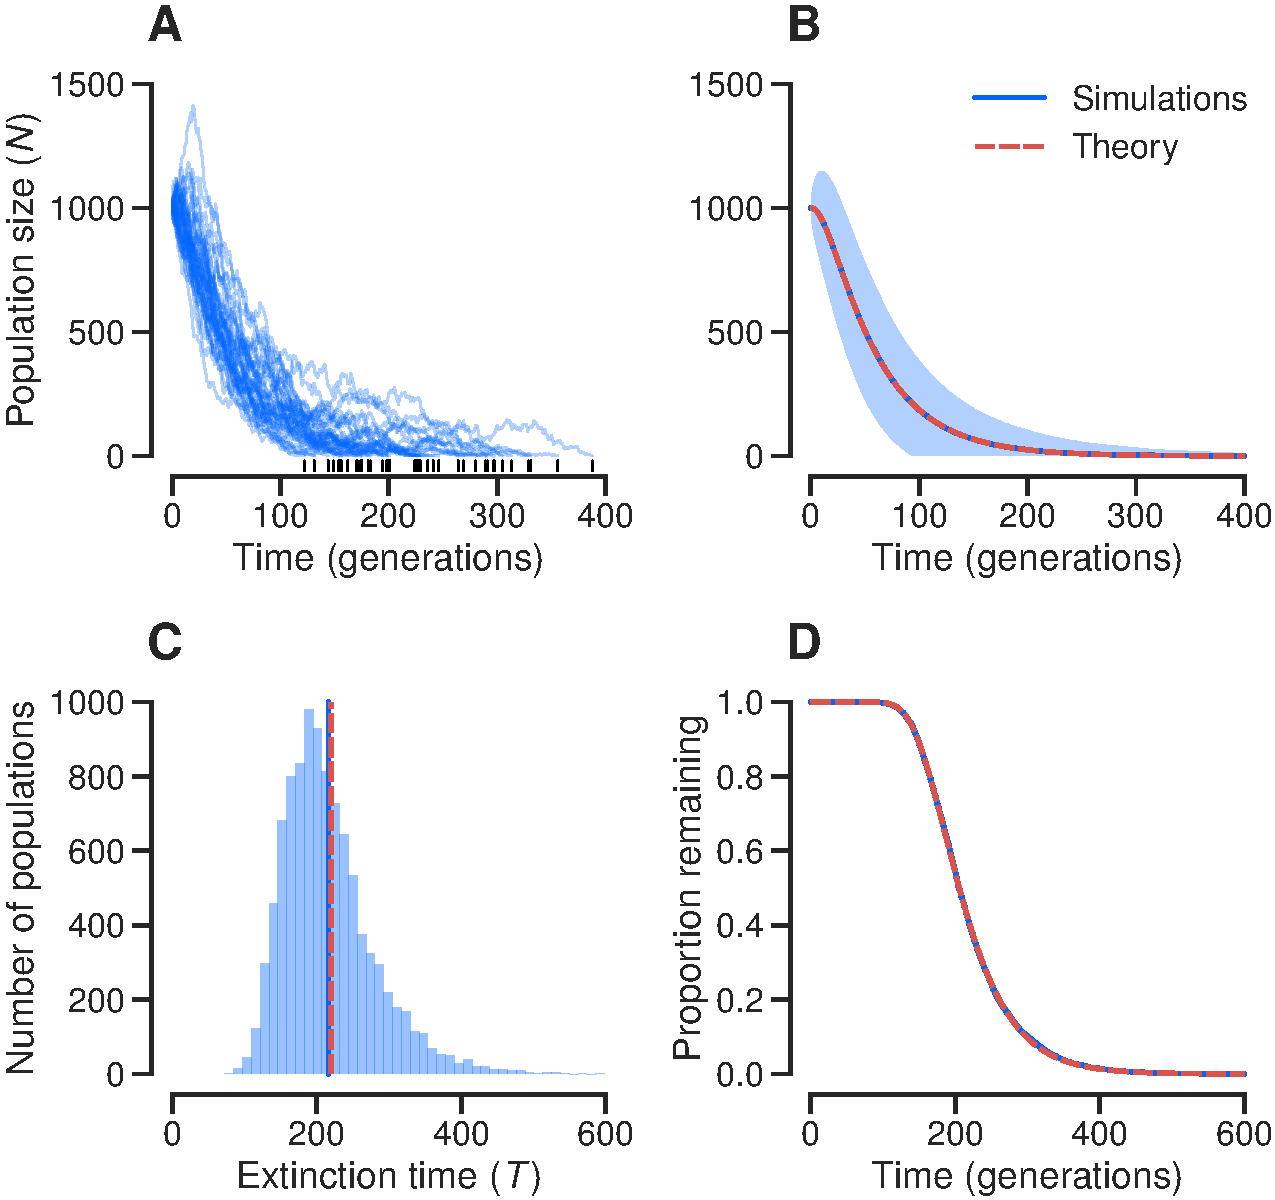
\includegraphics[width=.67\linewidth]{figures/fig2.pdf}
\caption{Populations are doomed to extinction in our model.  
%
\textbf{(A)} Dynamics of population size, $N$, in 40 populations founded by $n_0=100$ mutation-free individuals and subject to mutations with deleterious effect $s=0.01$ and rate $u=0.01$.  Black vertical lines above the time axis indicate extinction times.
%
\textbf{(B)} Blue line shows mean $N$ based on stochastic simulations of $10^4$ replicate populations like those shown in \textbf{(A)}.  
Light blue region indicates $\overline{N} \pm \mathrm{SD}[N]$ (standard deviation). If $\mathrm{SD}[N] > \overline{N}$, the lower bound of the region was set to zero.  
Red dashed line indicates expected population size (\EQ{N}).
%
\textbf{(C)} Distribution of extinction times, $T$, in the stochastic simulations described in \textbf{(B)}. 
Blue line shows mean $T$ based on the $10^4$ replicate populations.  
Red line shows $\mathbf{T}$ calculated numerically (see \textbf{Materials and Methods}).  
%
\textbf{(D)} Extinction times of populations with the same mutational parameters as those in \textbf{(A)} but with a range of initial populations sizes, $n_0$.
%
Blue line shows mean values of $T$ based on stochastic simulations of $10^4$ replicate populations for 41 values of $n_0$ evenly spaced on a log-scale over 4 orders of magnitude.
%
Light blue region indicates $\overline{T} \pm  \mathrm{SD}[T]$. If $\mathrm{SD}[T] > \overline{T}$, the lower bound of the region was set to zero.  See \FIGSUPP[decay]{sf1} for more on the variability of $T$.
%
Red line shows $\mathbf{T}$ calculated numerically.}
\label{fig:decay}
\figsupp[Variability of extinction time declines with population size.]{\textbf{Variability of extinction time declines with population size.}
%
Blue circles show coefficient of variation of $T$, CV$[T]$, for the data shown in \FIG{decay}D.  Red line shows CV$[T]$ calculated numerically using \EQ{CV}.}{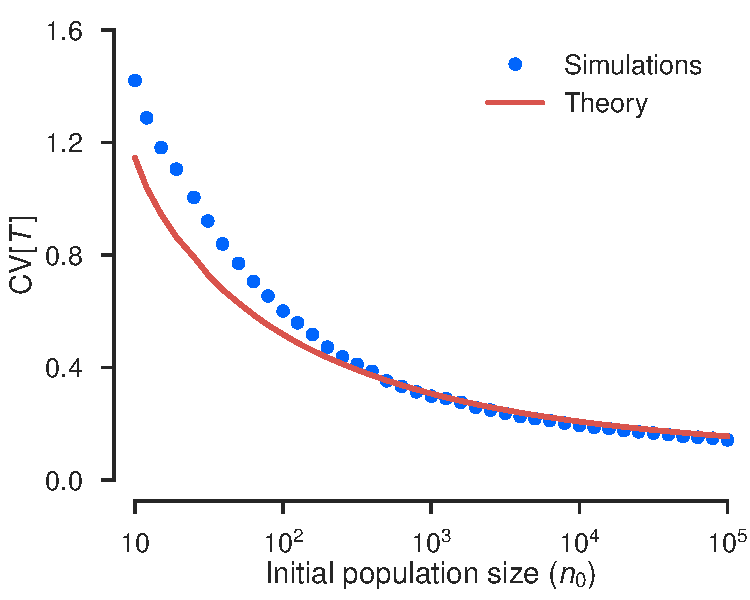
\includegraphics[width=0.39\linewidth]{figures/fig2s1.pdf}}\label{figsupp:sf1}
\end{figure}


\subsection{Large initial population size}


The expected time to extinction of the mutation-free class, $t_0$, is given by \EQ{t0}.
Following \citet{Jagers_On_2007}, there exists a sequence $c(n_0)\to c$ as $n_0\to\infty$ such that
%
\begin{equation}
t_0 = -\frac{\ln n_0 + c(n_0)}{\ln m_{0,0}} \quad ,
\label{eq:jagers}
\end{equation}
%
where $m_{0,0} = 1-u <1$ (\EQ{m}) is the expected number of mutation-free offspring per mutation-free individual and $n_0$ is the initial number of mutation-free individuals.  Note that the value of $c$ depends on $u$ (e.g., for $u=0.01$ and 0.02, numerical estimates using \EQ{t0} and \EQ{jagers} yield $c=3.3737$ and $2.7058$, respectively).

\EQ{jagers} shows that $t_0$ grows logarithmically with $n_0$ 
with a slope of $-1/\ln m_{0,0}$.  If $u$ is small, the slope becomes $\approx 1/u$.  Thus, increasing initial population size delays extinction of the mutation-free class more when the mutation rate is low than when it is high.

The value of $t_0$ is not affected by the effects of mutations, $s$ (\EQ{t0} and \EQ{jagers}), because the rate at which individuals ``leave'' the mutation-free class is independent of $s$.  The selection coefficient does, however, affect the size of the new least-loaded class (i.e., individuals with $k=1$ mutation), $x_1$ (\EQ{xk}), and therefore the total time to extinction. 

We now investigate the limiting behavior of $x_1$ as $n_0\to\infty$. By \EQ{xk} and \EQ{jagers} we get 

\begin{align}
%
x_{1} &\approx n_0 \, g_{1}(t_0) \nonumber \\[3pt]
      &= \frac{C(n_0) u}{s(1-u)} \left(1-(1-s)^{t_0}\right) \nonumber \\[3pt]
      &\to \frac{C u}{s(1-u)}
%
\label{eq:x1}
\end{align}
%
as $n_0\to\infty$, where $C(n_0) = e^{c(n_0)}$. If $u$ is small and $n_0$ is large, 
\EQ{x1} becomes $x_1 \approx C u / s$.
Interestingly, \EQ{x1} shows that $x_1$ approaches a constant as $n_0$ increases.


\begin{figure}[ht!]
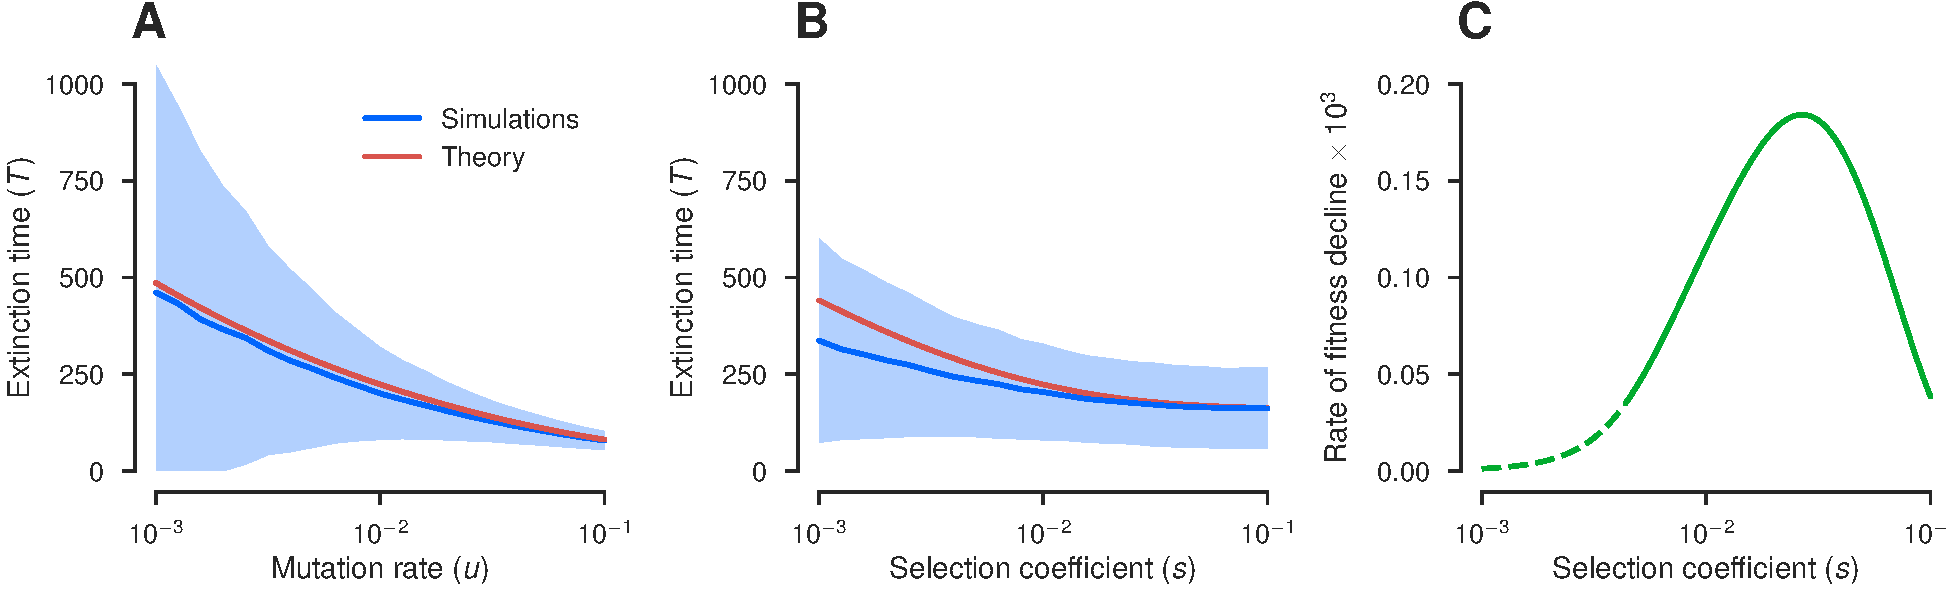
\includegraphics[width=\linewidth]{figures/fig3.pdf}
\caption{
Mutational parameters have different effects on extinction time in doomed populations and the severity of Muller's Ratchet in populations of constant size.
%
\textbf{(A--B)} Values are mean extinction times, $T$, in populations founded by $n_0=100$ mutation-free individuals but with different mutational parameters.  
%
\FIGSUPP[valid]{sf2} shows the variability of $T$.
%
\textbf{(A)} Mutations have deleterious effect $s=0.01$ and a range of mutation rates, $u$.
%
\textbf{(B)} Mutations occur with $u=0.01$ and have a range of values of $s$.
%
Blue lines show mean values of $T$ based on stochastic simulations of $10^4$ replicate populations for 21 values of the parameter being manipulated, evenly spaced on a log-scale.
%
Light blue regions indicate $\overline{T} \pm  \mathrm{SD}[T]$  If $\mathrm{SD}[T] > \overline{T}$, the lower bound of the region was set to zero.
%
Red lines show $\mathbf{T}$ calculated numerically (see \textbf{Materials and Methods}) for 41 values of the parameter being manipulated, evenly spaced on a log-scale.
%
\FIGSUPP[valid]{sf3} shows that the theoretical predictions for low $s$ become more accurate with increasing population size. 
%
\textbf{(C)} Severity of Muller's Ratchet in populations of constant size and a deleterious mutation rate of $U = 0.01$ per genome per generation.  Values are the expected declines in mean fitness per thousand generations, $10^3 \times s/\Delta t$, for 101 values of $s$ evenly spaced on a log-scale.  
$\Delta t$ is the time between clicks of the Ratchet calculated using the method of \citet{Gordo_On_2000, gor00b}.
Dashed and solid lines indicate $\hat n_k < 10$ and $\hat n_k \geq 10$, respectively (\EQ{haigh}).  
%
The trend shown in \textbf{(C)} was confirmed by simulation (not shown).
}
\label{fig:valid}
%
\figsupp[Variability of extinction time declines with mutation rate and is approximately invariant with selection coefficient.]{\textbf{Variability of extinction time declines with mutation rate and is approximately invariant with selection coefficient.}
%
Blue circles show coefficient variation of $T$, CV$[T]$, for the data shown in the corresponding panel of \FIG{valid}.  Red line shows CV$[T]$ calculated numerically using \EQ{CV}.}{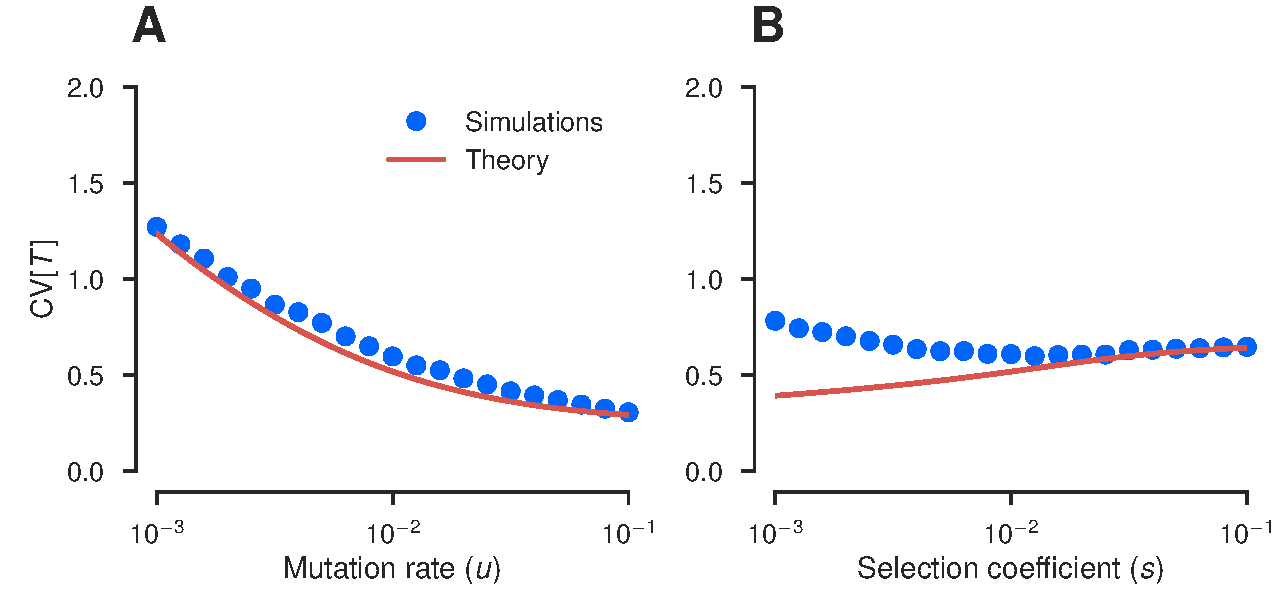
\includegraphics[width=0.67\linewidth]{figures/fig3s1.pdf}}\label{figsupp:sf2}
%
\figsupp[Theoretical predictions for low $s$ become more accurate with increasing population size.]{\textbf{Theoretical predictions for low $s$ become more accurate with increasing population size.}
%
\textbf{(A)} Extinction times of populations with $u=0.01$ and $s=10^{-3}$ over a range of initial populations sizes, $n_0$.
%
Blue line shows mean values of $T$ based on stochastic simulations of $10^4$ replicate populations for 41 values of $n_0$ evenly spaced on a log-scale over 4 orders of magnitude.
%
Light blue region indicates $\overline{T} \pm  \mathrm{SD}[T]$. If $\mathrm{SD}[T] > \overline{T}$, the lower bound of the region was set to zero.  
%
\textbf{(B)} Variability of extinction times shown in \textbf{(A)}. Blue circles show coefficient variation of $T$, CV$[T]$.  Red line shows CV$[T]$ calculated numerically using \EQ{CV}.}{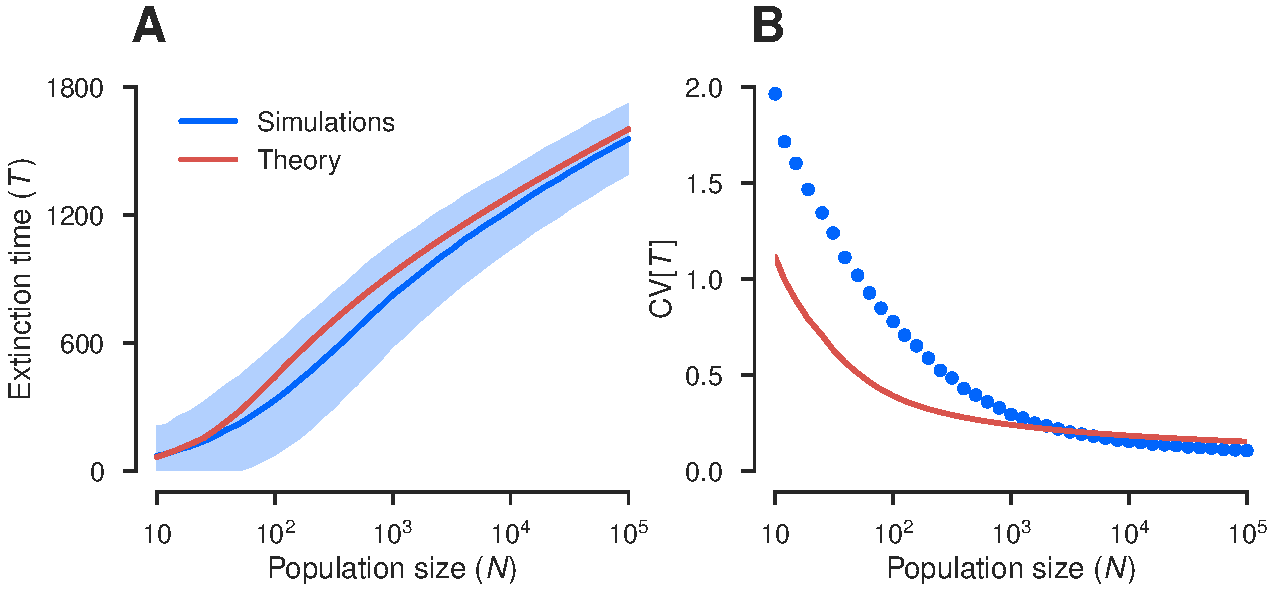
\includegraphics[width=0.67\linewidth]{figures/fig3s2.pdf}}\label{figsupp:sf3}
\end{figure}


\subsection*{Change in population size}


If a population is founded by $n_0$ mutation-free individuals, the expected total population size $t$ generations later is
%
\begin{equation}
E\left[N(t)\right] = n_0 \sum_{j=0}^t{g_{j}(t)}      
\label{eq:N} %\nonumber\\[2pt]
\end{equation}
%
(see \EQ{gj}).

Initially, $N(0) = n_0$.  Since all individuals have the same fitness, the population size is not expected to change in the following generation: $E\left[N(1)\right] = n_0$.  One generation later, the population size is expected to decline by $E\left[N(2)\right] - E\left[N(1)\right] = - n_0us$.  In subsequent generations, if mutations have small effects, the population size is expected to continue to decline at approximately the same rate
%
\begin{equation}
E\left[N(t+1)\right] - E\left[N(t)\right] \approx -n_0 u s t \quad .
\label{eq:deltaN}
\end{equation}




\section{Results}




\subsection{Small population size, high mutation rate, and mutations of large effect accelerate extinction}

In our model, population size, $N$, can increase as well as decrease from generation to generation.  However, all increases are transient and the population will eventually go extinct (\FIG{decay}A).  The expected value of $N$ can be predicted accurately by \EQ{N} (\FIG{decay}B).  However, the dynamics of the expected value of $N$ are not sufficient to predict the time to extinction.  Two populations with different initial population sizes, $n_0$, will be expected to show the same $N/n_0$ at any time (because they will have the same $g_j(t)$, \EQ{N}), but the smaller population is expected to go extinct earlier (\FIG{decay}C and \FIG{decay}D).  \EQ{T} provides good estimates of expected extinction time, $\mathbf{T}$, and variability in extinction time, over a broad range of initial population sizes, $n_0$ (\FIG{decay}D, \FIGSUPP[decay]{sf1}, and \FIGSUPP[valid]{sf3}), and mutational parameters (\FIG{valid}A, \FIG{valid}B, and \FIGSUPP[valid]{sf2}).  
(See \autoref{app:jensen} for an explanation of why \EQ{T} tends to overestimate the true value of $\mathbf{T}$.)  
Below, we focus on the numerical calculations of $\mathbf{T}$ based on \EQ{T}.

Our model has three parameters---$n_0$, $u$, and $s$---and all of them influence extinction time.  Smaller populations tend to go extinct faster.  \FIG{decay}D and \FIGSUPP[valid]{sf3}A show that $\mathbf{T}$ is approximately proportional to the logarithm of the initial population size, $n_0$.  
%
When $n_0$ is large, $t_0 \propto \ln n_0$ (\EQ{jagers}) and $x_1$ is approximately constant (\EQ{x1}).
Thus, 
$\Delta t_1, \Delta t_2, \ldots$ (\EQ{deltat})
are also expected to approach constant values as $n_0\to\infty$.  Since
$t_0$ grows logarithmically, this result implies that $t_0$ represents an increasing fraction of $\mathbf{T}$ as $n_0$ increases. 
Therefore, we also expect $\mathbf{T}$ to grow logarithmically with $n_0$. 
Variability in extinction time declines with $n_0$ (\FIGSUPP[decay]{sf1}).

At a particular value of $n_0$, however, $t_0$ is not sufficient to explain the variation in total extinction time for different mutational parameters: 
$t_0$ dominates $\mathbf{T}$ when $u/s$ is low, but not when it is high (\FIG{heat}B and \FIGSUPP[heat]{sf4}A).  One reason for this pattern is that $x_1$ increases with $u/s$ (\EQ{x1}; \FIG{heat}C).

Mutations cause extinction in our model, but how do they influence extinction \textit{time}?  
%
One possibility is that $\mathbf{T}$ is determined by the severity of Muller's Ratchet. High mutation rate and mutations of large effect accelerate extinction in doomed populations (\FIG{valid}A, \FIG{valid}B, and \FIG{heat}A).  Mutational parameters act differently on Muller's Ratchet in populations of constant size: at certain mutation rates the severity of the Ratchet is maximal at intermediate mutational effects \citep{Gabriel_MULLER_1993, Gordo_On_2000, gor00b} (\FIG{valid}C).
%
There are two possible explanations for this discrepancy.  
%
First, the Ratchet may operate differently in doomed populations and populations of constant size. 
%
Second, Muller's Ratchet may not determine extinction time in doomed populations.  
%
We explore each of these possibilities in the next two sections.  


\begin{figure}[ht!]
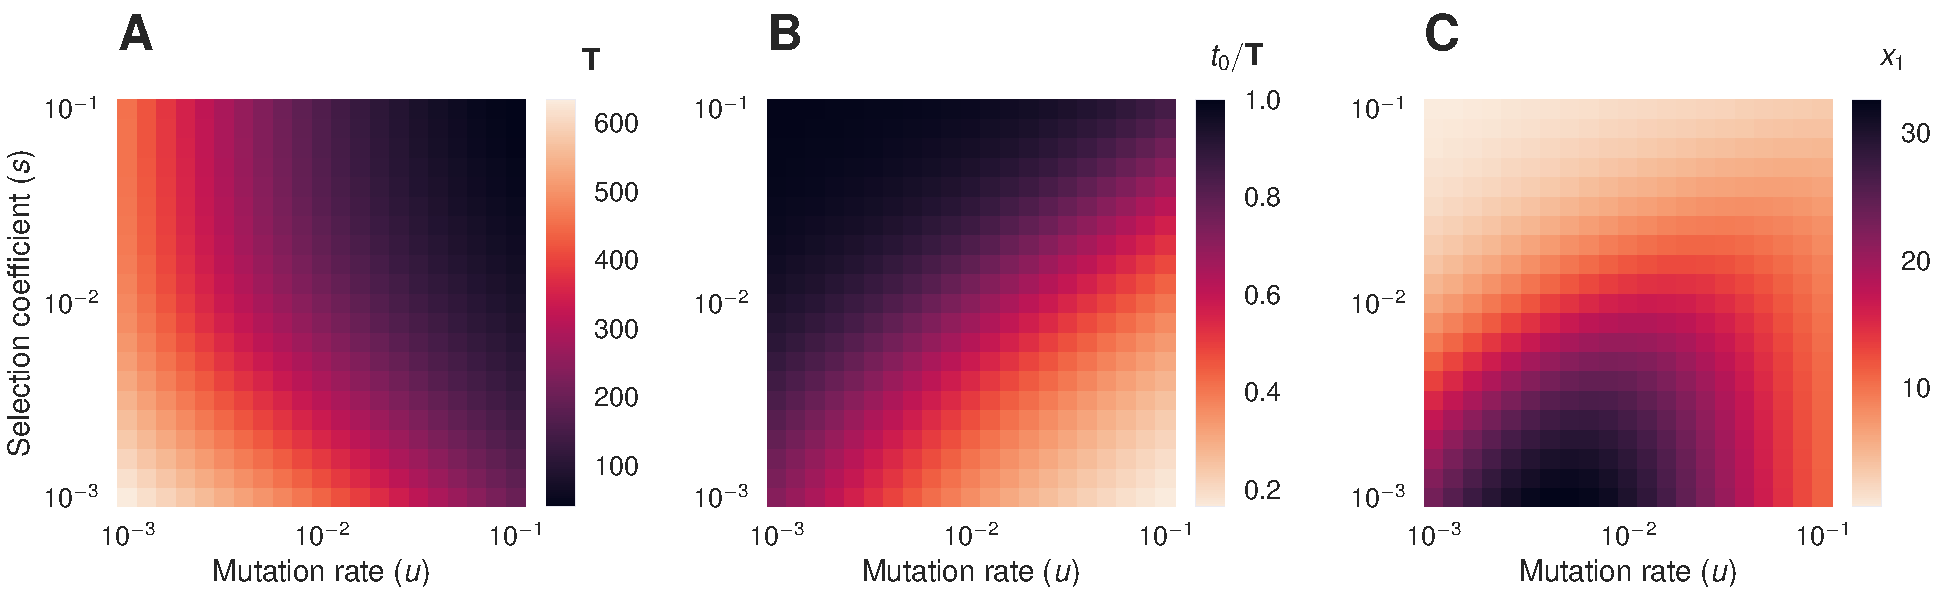
\includegraphics[width=\linewidth]{figures/fig4.pdf}
\caption{High mutation rate and mutations of large effect accelerate extinction in doomed populations.  
%
\textbf{(A)} Expected extinction time, $\mathbf{T}$, of populations founded by $n_0=100$ mutation-free individuals and subject to mutations with deleterious effect $s$ and rate $u$.  $\mathbf{T}$ was calculated numerically (see \textbf{Materials and Methods}) for $21\times21=441$ combinations of values of $s$ and $u$ evenly spaced on a log-scale.  (See \FIGSUPP[heat]{sf4}B for the variability of $T$.)
%
\textbf{(B)} Expected extinction time of the mutation-free class, $t_0$, as a proportion of $\mathbf{T}$ for the populations shown in \textbf{(A)}.  
$t_0$ was calculated numerically (see \textbf{Materials and Methods}).
\FIGSUPP[heat]{sf4}A shows $t_0$.
%
\textbf{(C)} Expected number of individuals with $k=1$ mutation at $t_0$, $x_1$ (\EQ{xk}), for the populations shown in \textbf{(A)}.
}
\label{fig:heat}
\figsupp[Expected extinction time of the mutation-free class and variability of extinction time.]{\textbf{Expected extinction time of the mutation-free class and variability of extinction time.}
%
\textbf{(A)} Expected extinction time of the mutation-free class, $t_0$, used in \FIG{heat}B.
%
\textbf{(B)} Coefficient of variation of $T$, CV$[T]$, calculated numerically using \EQ{CV}.}{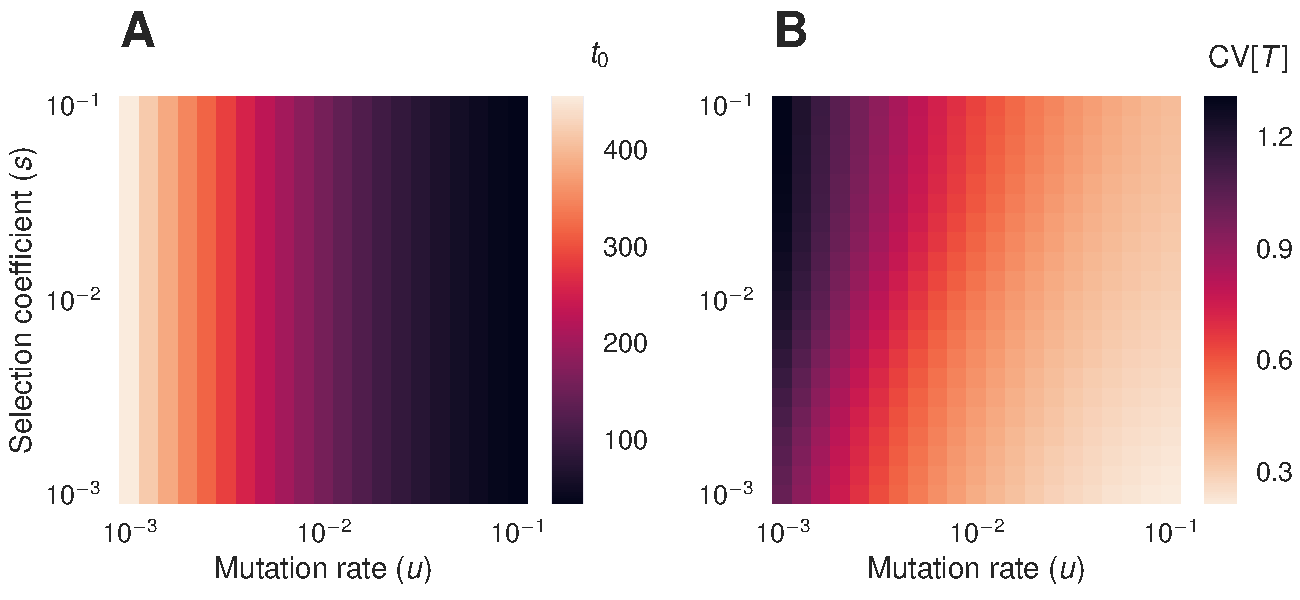
\includegraphics[width=0.67\linewidth]{figures/fig4s1.pdf}}\label{figsupp:sf4}
\end{figure}


\subsection{Low mutation rate and mutations of large effect accelerate mutational meltdown}


Lynch and colleagues have proposed that Muller's Ratchet accelerates in a doomed population as population size declines, driving the population to extinction---a phenomenon they called mutational meltdown \citep{Lynch_MUTATION_1990, lyn93, Gabriel_MULLER_1993}.  
Do our doomed populations experience mutational meltdown?

To answer this question we need a way to quantify the rate of mutational meltdown.  Let 
%
\begin{equation}
\Delta t_k = \left\{\begin{array}{lll}
%
    t_0               & , & k = 0       \\ [4pt]
	t_k - t_{k-1}     & , & k > 0
    \end{array}
%
\right. 
\label{eq:deltat}
\end{equation}
%
be the interval between clicks $k-1$ and $k$ of the Ratchet, where $t_k$ denotes the time of the $k$-th click.  
%
In populations of constant size, 
the Ratchet is expected to click at a steady rate over time, that is,
$\Delta t_k$ is not expected to change with $k$ \citep{Haigh_The_1978, Gordo_On_2000, gor00b}.  
%
In contrast, under mutational meltdown
the Ratchet is expected to accelerate in successive clicks, that is,
$\Delta t_k$ is expected to decline with $k$.
%
We find that $\Delta t_k$ declines approximately exponentially with $k$ in doomed populations (\FIG{melt}A).  Thus, we use the rate of this decline, $\beta$, to measure the rate of mutational meltdown.

Mutational parameters have large effects on the rate of mutational meltdown.  Low mutation rate and mutations of large effect accelerate mutational meltdown (\FIG{melt}).  This result is consistent with the effects of mutational parameters on $\Delta t_0$ and $\Delta t_1$ in large populations (\EQ{jagers} and \EQ{x1}).  
%
Low values of $u$ increase $\Delta t_0$  and decrease $x_1$, and therefore $\Delta t_1$, causing mutational meltdown to accelerate.  
%
High values of $s$ have no effect on $\Delta t_0$ but decrease $x_1$, and therefore $\Delta t_1$, also causing the meltdown to accelerate.


\begin{figure}[ht!]
\centering
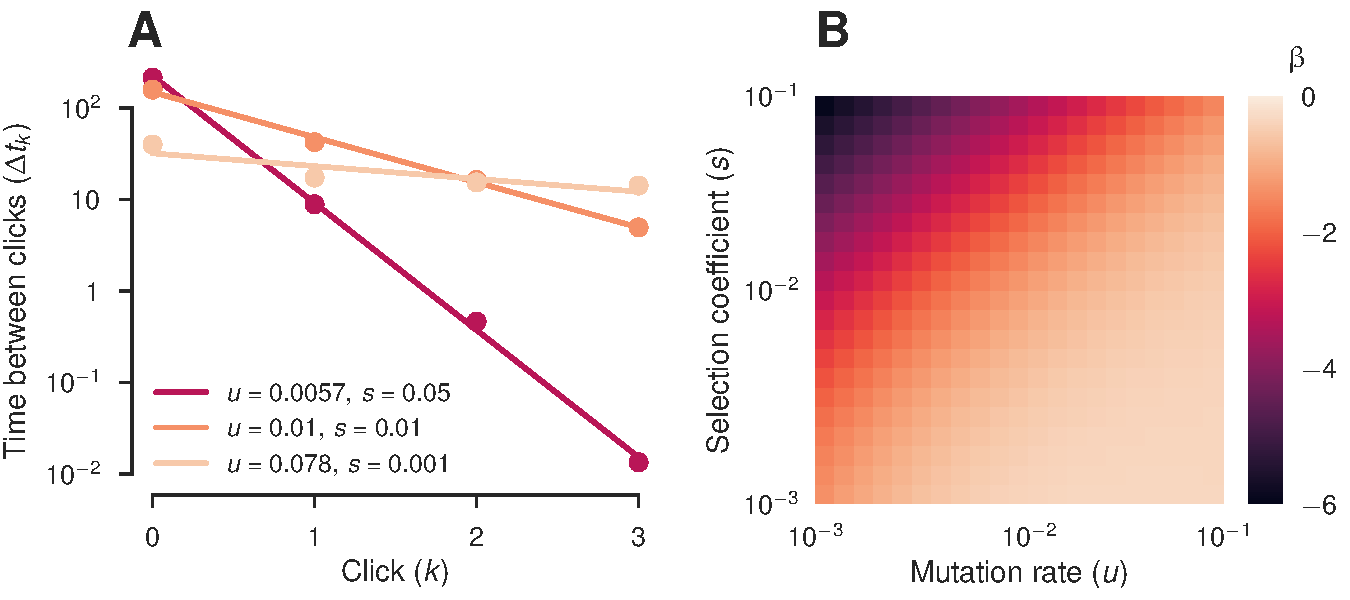
\includegraphics[width=.71\linewidth]{figures/fig5.pdf}
\caption{Mutational meltdown does not determine extinction time in doomed populations.  
%
\textbf{(A)} Circles denote time between clicks, $\Delta t_k$ (\EQ{deltat}).  Click $k$ indicates the extinction of $k$-type individuals.  Values of $t_0$ were calculated using \EQ{t0}; values of $t_1, t_2,$ and $t_3$ were calculated using \EQ{tk} (see \textbf{Materials and Methods}).
Note that $\Delta t_k$ is displayed on a log-scale.  Each combination of mutational parameters results in populations having the same expected extinction time $(\mathbf{T} = 223.52)$.  Lines indicate linear regression fits of $\ln \Delta t_k$ on $k$ (meltdown rates: $\beta = -3.20, -1.14$ and $-0.32$, respectively).
%
\textbf{(B)} Meltdown rates, $\beta$, calculated as shown in \textbf{(A)} for $21\times21=441$ combinations of values of $s$ and $u$ evenly spaced on a log-scale.
}
\label{fig:melt}
\end{figure}


\subsection{Extinction time is determined by the rate of fitness decline}


Does mutational meltdown determine extinction time? 
%
\FIG{melt} shows that doomed populations can experience strong mutational meltdown.  However, mutational meltdown does not determine extinction time.  Although the three scenarios summarized in \FIG{melt}A have widely different meltdown rates, they have the same expected extinction time, $\mathbf{T} = 223.52$.  The lack of correlation between $\mathbf{T}$ and $\beta$ is clear when we compare \FIG{heat}A and \FIG{melt}B.
Although the meltdown rate does not determine extinction time,
for a given extinction time, the meltdown rate is positively correlated with the \textit{variability} in extinction time (\FIGSUPP[valid]{sf2} and \FIGSUPP[heat]{sf4}B).

The results so far indicate that Muller's Ratchet does not determine extinction time in doomed populations.  So what does?
%
Extinction is, trivially, caused by decline in population size.  In our model the rate of decline in population size is determined by the \textit{product} of mutation rate and effect, $us$ (\EQ{deltaN}).  This makes intuitive sense because the rate of decline in population size is determined by the absolute fitness of individuals and both $u$ and $s$ are inversely related to fitness: 
increasing $s$ reduces the fitness of an individual directly (\EQ{fit}) and increasing $u$ reduces the fitness of an individual's offspring.
%
This explains why time to extinction declines with both $u$ and $s$ (\FIG{heat}A).




\section{Discussion}




Most models of Muller's Ratchet have assumed that populations maintain a constant size as deleterious mutations accumulate \citep{Haigh_The_1978, Gessler_The_1995, Gordo_On_2000, gor00b, Rouzine_The_2003, met13}.
This is typically justified as resulting from density-dependent regulation of population size.  
However, the assumption is unrealistic because it prevents populations from ever going extinct \citep{Lynch_MUTATION_1990, mel91}.  
%
In a series of studies relaxing the assumption of constant population size, Lynch, Gabriel, and colleagues argued that Muller's Ratchet eventually generates a positive feedback where
the Ratchet clicks, 
which causes population size to decline, 
which strengthens genetic drift relative to natural selection,
which in turn accelerates the Ratchet \citep{Lynch_MUTATION_1990, lyn93, Gabriel_MULLER_1993}.  
They called this vicious cycle mutational meltdown and concluded that it drives populations to extinction.  
However, the lack of quantitative theory on the mutational meltdown has made it difficult to evaluate the Lynch-Gabriel hypothesis.

Our results challenge the Lynch-Gabriel hypothesis.  Although doomed populations can experience mutational meltdown---measured by the acceleration of Muller's Ratchet---, the rate of mutational meltdown does not determine extinction time (\FIG{melt}A).  Therefore, the Lynch-Gabriel mutational meltdown is not a general \textit{cause} of extinction.  Rather, our results suggest that extinction time is determined by the expected impact of deleterious mutations on fitness.  
Interestingly, if we compare populations with the same expected extinction time but different mutational parameters, populations undergoing faster meltdown rate have more variable extinction times than populations undergoing slower meltdown  (\FIGSUPP[heat]{sf4}).

The Lynch-Gabriel hypothesis emphasized the role of the change in the strength of genetic drift in causing mutational meltdown \citep[e.g., ``we refer to this synergism between mutation accumulation and random genetic drift as a mutational meltdown'';][]{lyn93}.  
Our results indicate that extinction in doomed populations is driven by mutation pressure, not genetic drift.  
%
\citet{Gessler_The_1995}  identified a related phenomenon in the operation of Muller's Ratchet under constant population size: if the mutation rate is too high the Ratchet is driven by mutation pressure, not genetic drift.
%
Since the expression ``mutational meltdown'' is now in common usage \citep[e.g.,][]{poo00, row03, Allen_Mutational_2009, McFarland_Tug_2014}, we propose that it be revised to refer to extinction caused by mutation pressure.

The extent to which real populations undergo mutational meltdown is unclear.  A population must first enter the doomed regime.  Models of Muller's Ratchet in populations of constant size
have identified three major risk factors that can drive populations into the doomed regime: long-term reductions in population size,  increases in mutation rate, 
and intermediate deleterious effects of mutations
\citep{Lynch_MUTATION_1990, lyn93, Gabriel_MULLER_1993, lyn95, McFarland_Impact_2013}.  Increased mutation rate can even drive a very large population into the doomed regime---a phenomenon known as lethal mutagenesis \citep{Bull_Theory_2007}.
Next, we consider the first two risk factors..

Population size can decline as a result of changes in the environment, such as, climate change, decreased food availability, emergence of infectious diseases, and habitat loss or fragmentation.  
For example, the emergence of Devil Facial Tumor Disease, a transmissible cancer, has caused the size of the Tasmanian devil population to decline by $\sim$77\% within 5 years \citep{haw06, laz18}.  As a result, the devils are under risk of extinction \citep{mcc09}. 
%
Our results indicate that increasing population size causes relatively small delays in extinction in doomed populations.  
%
$\mathbf{T}$ is approximately proportional to the logarithm of initial population size (\FIG{decay}D).  
%
Similar results have been obtained in other stochastic models of population dynamics \citep{lan93, Jagers_On_2007}.

Increases in mutation rate have been observed directly in experimental populations.  For example, a population of \emph{Escherichia coli} adapting to a constant environment evolved a mutator mutation after $\sim$25,000  generations that increased mutation rate by $\sim$150-fold \citep{bar09, wie13}.
%
Evolution experiments have revealed that real populations can, indeed, experience  increased extinction risk when the mutation rate is high.  
%
\citet{zey01a} allowed 12 populations of the yeast \textit{Saccharomyces cerevisiae} with genetically elevated mutation rate to evolve and found that two of them went extinct within 2,900 generations.  One of these populations went extinct shortly after a large decline in fitness.
%
\citet{ban16} subjected two populations of influenza A virus to gradually increasing concentrations of favipiravir, a drug that increases the mutation rate of the virus, and observed that both populations accumulated mutations rapidly and went extinct. 
%
The results from both of these studies are broadly consistent with the occurrence of a mutational meltdown.  However, they do not allow us to distinguish between the Lynch-Gabriel model and ours.

The results described in the previous paragraph indicate that mutational meltdown might have clinical applications.  
%
Mutagenic agents are being explored as antiviral drugs \citep{loe99, cro01, par01, ban16}.
%
Increased mutation rate in tumor cells has been found to correlate with improved outcomes for some cancers \citep{sil00, bir11, and16}.  
%
Several inhibitors of key components of the DNA-repair and DNA damage-response machinery \citep[e.g., PARP inhibitors,][]{lor15}, are currently being used to treat cancer, or are under preclinical or clinical development \citep{bro17}.

The relative theoretical neglect of the evolutionary dynamics in doomed populations is surprising given that it is central to understanding the long-term consequences of both Muller's Ratchet \citep{Lynch_MUTATION_1990,lyn93,Gabriel_MULLER_1993,lyn95} and lethal mutagenesis \citep{Bull_Theory_2007, mat17}.  
%
In both cases, the duration of the meltdown phase was dismissed because it was predicted to be short relative to the time required for the population to \textit{become} doomed \citep{lyn93,lyn95,Bull_Theory_2007}.
%
We believe that this neglect of the meltdown phase is misplaced because it is an important phase in the life of a population---the last chance for the population to be rescued by beneficial mutations and avoid extinction.  The dynamics and duration of the meltdown phase are expected to be important determinants of the probability of evolutionary rescue.  For a given probability of beneficial mutation and selection coefficient of those mutations, populations that decline in size more slowly and retain higher proportions of mutation-free individuals for longer, are more likely to be rescued \citep{mar13}.  
%
Rescue of doomed populations may play an important role in cancer progression \citep{McFarland_Impact_2013, McFarland_Tug_2014}.

A central assumption of our model  is that individuals experience hard selection \citep{wal75}.   
The expected number of offspring of an individual is its absolute fitness, $w_k$ (\EQ{fit}), and is both density independent and frequency independent.  The Lynch-Gabriel models make similar assumptions during the mutational meltdown phase \citep{lyn93,lyn95}. 
% 
In contrast, classic models of Muller's Ratchet typically assume soft selection \citep{wal75}.  Constant population size implies density dependence.  Selection is also frequency dependent: the expected number of offspring of an individual depends not only on its fitness, but on the fitness of other individuals in the population.
%
The difference in the mode of selection in these models explains the different effects of the deleterious effect of a mutation, $s$, on extinction time in our model, and on the severity of Muller's Ratchet in classic models.  In doomed populations, increasing $s$ accelerates extinction, albeit with diminishing returns (\FIG{decay}B and \FIG{heat}).  In models with soft selection, the Ratchet is most severe at an intermediate value of $s$ 
\citep[\FIG{decay}C;][]{lyn95, Gordo_On_2000, gor00b}.  

In reality, populations do not necessarily experience either of the extremes of soft or hard selection.  Factors such as population structure, resource availability, and the mechanism of competition can modulate the ``softness'' of selection in complex ways; different genotypes in a population, and even different genes, can experience different softness of selection \citep{laf10, ho12}.  This raises the interesting question of how mutational meltdown operates in regimes of intermediate softness, or with a smooth transition between soft and hard selection as mutations accumulate.

Our model includes at least three other simplifications that could have important consequences for the evolutionary dynamics of doomed populations.  
%
First, the environment, and therefore selection, is constant.  \citet{Wardlaw_Temporal_2012} showed that temporal variation in selection can accelerate Muller's Ratchet in populations of constant size.
%
Second, all mutations are deleterious.  Beneficial mutations could, potentially, rescue a population from extinction \citep{mar13}.  Furthermore, compensatory mutations might become more common as fitness declines \citep{poo00, sil07}.
%
Third, individuals reproduce asexually.  Sex has been shown to slow down Muller's Ratchet dramatically in populations of constant size \citep{pam87, cha93}, and can delay extinction in large populations \citep{lyn95a}.
%
We believe that our model provides a promising framework to explore the consequences of relaxing these assumptions 
for the fate of populations doomed to extinction.




\section{Materials and Methods}




\subsection{Numerical calculations}

\subsubsection{Expected extinction time of the mutation-free class}
We calculated $t_0$ by computing \EQ{t0} until the following criterion was met 
%
\[ \left(\varphi_{k}^{(t)}(0)\right)^{n_{0}} - \left(\varphi_{k}^{(t+1)}(0)\right)^{n_{0}} < 10^{-6} \quad . \]
%
A similar criterion was applied when evaluating \EQ{vartauk} and \EQ{tk}. 

\subsubsection{Expected extinction time}
We calculated $\mathbf{T}=E[T]$ (\EQ{T}) by computing \EQ{tk} until the following criterion was met 
%
\[ t_k - t_{k-1} < 10^{-6} \quad . \]
%
We computed $\mathbf{T}$ for both bounds of $P(\tau_{k} > 0)$ when $k>0$ (\EQ{bounds}).  We present only results for the lower bound.  None of our conclusions would be changed if we used the upper bound results instead (not shown).

\subsubsection{Variance in extinction time}

We calculated the variance in extinction time by computing 
%
\begin{equation}
    \mathrm{Var}[T] = \sum_{k=0}^\infty \mathrm{Var}[\tau_k] \quad ,
    \label{eq:varT}
\end{equation}
%
up to the same value of $k$ used to calculate $\mathbf{T}$ (see \EQ{vartauk}).  
Again, we only present results for the lower bound of $P(\tau_{k} > 0)$ when $k>0$ (\EQ{bounds}).
\EQ{varT} assumes that the extinction times of different classes are independent (i.e., we ignore the covariance terms).  
This assumption was confirmed by simulations (not shown).

\subsubsection{Coefficient of variation in extinction time}

The coefficient of variation measures the variability of a variable relative to its mean. 
We calculated the coefficient of variation of extinction time by computing 
%
\begin{equation}
    \mathrm{CV}[T] = \frac{\sqrt{\mathrm{Var}[T]}}{\mathbf{T}} \quad . 
    \label{eq:CV}
\end{equation}


\subsection{Code availability}


Numerical calculations and stochastic simulations of the branching process model were done using software written in Python 2.7.
All code is available through \url{https://github.com/rbazev/doomed}.





\section{Acknowledgments}

We thank Alex Stewart, Ata Kalirad, Herbert Levine, and Erin Kelleher for helpful discussions.  

% Additional information can be given in the template, such as to not include funder information in the acknowledgments section.

\bibliography{bibliography}




%%%%%%%%%%%%%%%%%%%%%%%%%%%%%%%%%%%%%%%%%%%%%%%%%%%%%%%%%%%%
%%% APPENDICES
%%%%%%%%%%%%%%%%%%%%%%%%%%%%%%%%%%%%%%%%%%%%%%%%%%%%%%%%%%%%




\appendix


\begin{appendixbox}

\label{app:proof}
\section{Proof of \EQ{mt}}
Given real numbers $b$ and $x$ and $n \in \N$ (the nonnegative integers), let $A$ denote the ``almost diagonal'' $n \times n$ matrix
\[
A = \left( \begin{array}{ccccc} 1 & b \\ & x & bx \\ & & x^2 & bx^2 \\ & & & \ddots & \ddots \\ & & & & x^{n-1} \end{array} \right) \quad ,
\]
whose $i$th row is simply $x^{i-1}$ multiplied by $( \begin{array}{cccccccccc} 0 & 0 & \cdots & 0 & 1 & b & 0 & 0 & 0 & \cdots \end{array} )$, the 1 occuring in the $i$th position.  Since $A$ is upper triangular, so is its $k$th power (for $k \in \N$), with diagonal entries
\[
A^k(i,i) = x^{k(i-1)}.
\]
The superdiagonal entries aren't quite as simple, but can also be expressed explicitly in terms of $x$, $k$ and $b$.

\begin{lemma}\label{main}
For $n, k \in \N$, $1 \le i \le n-1$ and $1 \le j \le n-i$ one has
\[
A^k(i,i+j) = b^j x^{\frac{j(j-1)}{2} + k(i-1)} \prod_{\ell = 1}^{j} \frac{x^{k+1- \ell} - 1}{x^{\ell} - 1} \quad ,
\]
provided that we declare $x^0 = 1$.  
\end{lemma}

\begin{proof}
We induct on $k$.  When $k=1$, for $j=1$ and any $i$ the given expression becomes
\[
bx^{k(i-1)} \frac{x-1}{x-1} = bx^{(i-1)} = A(i,i+1) \quad .
\]
When $j \ge 2$, then the $\ell = 2$ factor in the product is $\frac{x^{2-2}-1}{x^2-1}=0$, so that regardless of $i$ the entire expression becomes $0$, which again equals $A(i,i+j)$.  We conclude that the stated result holds for $k=1$.

Now assume the result is true for some $k \ge 1$.  Since $A^{k+1} = A \cdot A^{k}$ and $A(i,\ell)=0$ unless $\ell \in \left\{ i , i+1 \right\}$,
\[
\begin{split}
A^{k+1}(i,i+j) &= \sum_{\ell=1}^n A(i,\ell) A^k(\ell, i+j) \\
  &= x^{i-1}A^k(i, i + j) + b x^{i-1}A^k(i+1,i+j) \\
  &= x^{i-1} \left( A^k(i,i+j) + bA^k(i+1,(i+1)+(j-1))) \right).
\end{split}
\]
Using the inductive hypothesis\footnote{Strictly speaking, the inductive hypothesis will only apply to the term $A^k(i+1,(i+1)+(j-1))$ when $j \ge 2$.  However, if we adopt the convention that any empty product is equal to one, the expression stated in the result agrees with $A^k(i+1,(i+1)+(j-1))$ when $j=1$ as well.} we obtain
\[
\begin{split}\hspace{-1.0cm}
& A^{k+1}(i, i+j)\\ 
& = b^j x^{i-1 + \frac{(j-1)(j-2)}{2}+ki} \left( \prod_{\ell=1}^{j-1} \frac{x^{k+1-\ell}-1}{x^{\ell}-1} \right) \left(x^{j-k-1}\frac{x^{k+1-j}}{x^j-1}+1  \right)\\
   &=b^j x^{i-1 + \frac{(j-1)(j-2)}{2}+ki} \left( \prod_{\ell=1}^{j-1} \frac{x^{k+1-\ell}-1}{x^{\ell}-1} \right) \left( \frac{1-x^{j-k-1}+x^j-1}{x^j-1}  \right)\\
   &=b^j x^{i-1 + \frac{(j-1)(j-2)}{2}+ki + j-k-1} \left( \prod_{\ell=1}^{j-1} \frac{x^{k+1-\ell}-1}{x^{\ell}-1} \right) \left( \frac{x^{k+1}-1}{x^j-1}  \right)\\
   &=b^j x^{\frac{j(j-1)}{2} + (k+1)(i-1)}  \left( \prod_{\ell=1}^{j-1} \frac{x^{k+1-\ell}-1}{x^{\ell}-1} \right) \left( \frac{x^{k+1}-1}{x^j-1}  \right) \\
   &=b^j x^{\frac{j(j-1)}{2} + (k+1)(i-1)}  \left( \prod_{\ell=1}^{j} \frac{1}{x^{\ell}-1} \right) \left(\prod_{\ell=0}^{j-1} (x^{k+1-\ell}-1)  \right) \\
   &= b^j x^{\frac{j(j-1)}{2} + (k+1)(i-1)}  \left( \prod_{\ell=1}^{j} \frac{x^{(k+1) + 1-\ell} -1}{x^{\ell}-1} \right), 
\end{split}
\]
\normalsize
which shows that the formula holds for the exponent $k+1$.  This concludes the proof.
\end{proof}

\end{appendixbox}


\begin{appendixbox}

\label{app:jensen}
\section{Overestimation of the Expected Extinction Time}

As shown in the \textbf{Model} section, an approximation is made in \EQ{approx} in order to derive analytical expressions for click times ($t_k$) and time to extinction (\textbf{T}). 
\FIG{decay}D, \FIG{valid}A, \FIG{valid}B, and \FIGSUPP[valid]{sf3}A show that the approximation is quite accurate over broad ranges of parameters but consistently overestimates \textbf{T}.

Overestimation of \textbf{T} is partly explained by the concavity of $E[\tau_k]$ as a function of $x_k$ in Equation \ref{eq:tauk}. 
The second derivative with respect to $x_k$ is 
\begin{equation*}
\frac{d^2E[\tau_k]}{d x_k^2} = -\sum \limits_{t=1}^\infty \left(\varphi_{k}^{(t)}(0)\right)^{x_{k}}\ln^2\left(\varphi_{k}^{(t)}(0)\right)
\end{equation*}
which is negative because both factors of each term in the sum are positive and hence the function is concave. By the reversed Jensen's inequality, for a concave function, $E[f(X)]<f(E[X])$, which implies that $E[\tau_k]$ is consistently overestimated by \EQ{tauk}.  Thus, \EQ{T} overestimates \textbf{T}. 

\end{appendixbox}

\end{document}
